\documentclass{article}
\usepackage{amsmath}
\usepackage[utf8]{inputenc}
\usepackage{graphicx}
\usepackage{verbatim}
\usepackage{float}
\usepackage[makeroom]{cancel}
\usepackage[english]{babel}
\usepackage{textcomp}
\usepackage{gensymb}
\usepackage{color}
\usepackage{subcaption}
\usepackage{caption}
\usepackage{hyperref}
\usepackage{physics}
\usepackage{dsfont}
%\usepackage{amsfonts}
\usepackage{listings}
\usepackage{multicol}
\usepackage{units}

\usepackage{algorithmicx}
\usepackage{algorithm}% http://ctan.org/pkg/algorithms
\usepackage{algpseudocode}% http://ctan.org/pkg/algorithmicx

\usepackage[margin=1cm]{caption}
\usepackage[outer=1.2in,inner=1.2in]{geometry}
% For writing full-size pages
%\usepackage{geometry}
%\geometry{
%  left=5mm,
%  right=5mm,
%  top=5mm,
%  bottom=5mm,
%  heightrounded,
%}

% Finding overfull \hbox
\overfullrule=2cm

\lstset{language=IDL}
 %\lstset{alsolanguage=c++}
\lstset{basicstyle=\ttfamily\small}
 %\lstset{backgroundcolor=\color{white}}
\lstset{frame=single}
\lstset{stringstyle=\ttfamily}
\lstset{keywordstyle=\color{red}\bfseries}
\lstset{commentstyle=\itshape\color{blue}}
\lstset{showspaces=false}
\lstset{showstringspaces=false}
\lstset{showtabs=false}
\lstset{breaklines}
\lstset{aboveskip=20pt,belowskip=20pt}

\lstset{basicstyle=\footnotesize, basewidth=0.5em}
\lstdefinestyle{cl}{frame=none,basicstyle=\ttfamily\small}
\lstdefinestyle{pr}{frame=single,basicstyle=\ttfamily\small}
\lstdefinestyle{prt}{frame=none,basicstyle=\ttfamily\small}
% \lstinputlisting[language=Python]{filename}


\definecolor{codepurple}{rgb}{0.58,0,0.82}
\definecolor{backcolour}{rgb}{0.95,0.95,0.92}
\definecolor{dkgreen}{rgb}{0,0.6,0}
\definecolor{gray}{rgb}{0.5,0.5,0.5}
\definecolor{magenta}{rgb}{0.58,0,0.82}

\lstdefinestyle{pystyle}{
  language=Python,
  aboveskip=3mm,
  belowskip=3mm,
  columns=flexible,
  basicstyle={\small\ttfamily},
  backgroundcolor=\color{backcolour},
  commentstyle=\color{dkgreen},
  keywordstyle=\color{magenta},
  numberstyle=\tiny\color{gray},
  stringstyle=\color{codepurple},
  basicstyle=\footnotesize,
  breakatwhitespace=false,
  breaklines=true,
  captionpos=b,
  keepspaces=true,
  numbers=left,
  numbersep=5pt,
  showspaces=false,
  showstringspaces=false,
  showtabs=false,
  tabsize=2
}

%%%%%%%%%%%%%%%%%%%%%%%%%%%%%%%%
% Self made macros here yaaaaaay
\newcommand\answer[1]{\underline{\underline{#1}}}
\newcommand\pd[2]{\frac{\partial #1}{\partial #2}}
\newcommand\redrum[1]{\textcolor{red}{\textbf{#1}}}
\newcommand\numberthis{\addtocounter{equation}{1}\tag{\theequation}}
% Usage: \numberthis \label{name}
% Referencing: \eqref{name}

% Some matrices
\newcommand\smat[1]{\big(\begin{smallmatrix}#1\end{smallmatrix}\big)}
\newcommand\ppmat[1]{\begin{pmatrix}#1\end{pmatrix}}

% Title/name/date
\title{AST4310 - Stellar Spectra A}
\author{Simen Nyhus Bastnes\\simennb}
\date{23. September 2016}

\begin{document}
\maketitle

\section{Introduction}\label{introduction}
In this project, we will look closer at the nature and appearance of spectral lines in stellar spectra. Doing so, we will retrace some of the steps of the early pioneers in the field of stellar spectroscopy.\\\\
First, we will take on the role of Cecilia Payne, and re-act the work on Saha-Boltzmann modeling of the Harvard classification. Then, we place our self in the role of Marcel Minnaert and his work on Schuster-Schwarzschild modeling of Fraunhofer line strengths.
%\section{Spectral classification}\label{spectral}
\section{Saha-Boltzmann calibration of the Harvard sequence}
In this section, we will attempt to explain the spectral-type sequence. In doing so, we will re-act the work of Cecilia Payne at Harvard. We will apply the Saha distribution for different ionization stages of an element to stellar spectra to find that the Harvard classification represents primarily a temperature scale.%\redrum{maybe rewrite cause very similar to SSA text :(}
%\subsection{Payne's line strength diagram}

\subsection{The Boltzmann and Saha laws}
First of all, we look at an energy level diagram for hydrogen.
\begin{figure}[H]
  \centering
  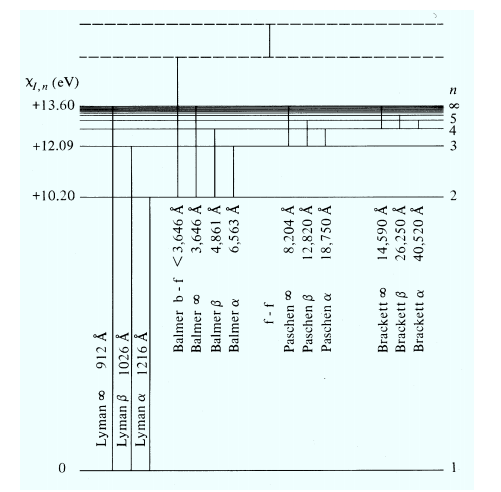
\includegraphics[scale=0.6]{figure7.png}
  \caption{Energy level diagram for hydrogen, taken from figure 7 in reference\cite{cite:ssa}}
  \label{fig:7}
\end{figure}
We see that some of the transitions share levels. The Balmer series all share the same lower level as each other, the Lyman series share the same lower level, the Paschen share lower level, and the Brackett share lower level, so one would assume that the series are defined based on all transitions to a common lower level.\\\\
When it comes to sharing higher levels, Balmer $\beta$ and Paschen $\beta$ share the same upper level, as do Balmer $\alpha$ and Lyman $\beta$. All of the series also have an $\infty$ transition that share the same ``upper level''.\\\\
Payne assumed that the strength of the absorption lines observed in stellar spectra scales with the population density of the lower level of the corresponding transition. Even though it is not correct, it would at first glance seem likely, as a higher lower level population would mean that there is a higher amount of particles that can be excited to a higher level, and then back down again. We will in this exercise follow her example, and assume that the scaling is linear.\\\\
With this, we can maybe attempt to give some rough estimates of the strength ratios of the $\alpha$ lines in the HI Lyman, Balmer, Paschen and Brackett series. Since Lyman $\alpha$ has a lower level in the ground state, we would assume that it would be the strongest of the lines, with Balmer being a far bit weaker than that, and Paschen and Brackett being consecutively weaker, but not as large difference due to the lower lever energy differensial decreasing the further up towards ionization we go.

\subsubsection*{Boltzmann law}
In TE the partitioning of a specific atom or ion stage over its discrete energy levels is given by the Boltzmann distribution
\begin{align*}
  \frac{n_{r,s}}{N_r} = \frac{g_{r,s}}{U_r}\,e^{-\chi_{r,s}/kT}\numberthis\label{eq:boltzmann}
\end{align*}
with $T$ the temperature, $k$ the Boltzmann constant, $n_{r,s}$ the number of particles per cm$^3$ in level $s$ of ionization stage $r$, $g_{r,s}$ the statistical weights of that level, and $\chi_{r,s}$ the excitation energy of that level measured from the ground state ($r,1$), $N_r \equiv\sum_sn_{r,s}$ the total particle density in all levels of ionization stage $r$, and $U_r$ its partition function defined by
\begin{align*}
  U_r = \sum_sg_{r,s}e^{-\chi_{r,s}/kT}
\end{align*}

\subsubsection*{Saha law}
In TE the particle partitioning over the various ionization stages of an element is given by the Saha distribution
\begin{align*}
  \frac{N_{r+1}}{N_r} &= \frac{1}{N_e}\frac{2U_{r+1}}{U_r}\bigg(\frac{2\pi m_ekT}{h^2}\bigg)^{3/2}\,e^{-\chi_r/kT} \numberthis\label{eq:saha}
\end{align*}
with $N_e$ the electron density, $m_e$ the electron mass, $h$ the planck constant, $chi_r$ the threshold energy needed to ionize stage $r$ to stage $r+1$, and $U_{r+1}$ and $U_r$ the partition function of ionization stages $r+1$ and $r$.

\subsection{Schadee's tables for schadeenium}
To test the Boltzmann and Saha laws, we look at a hypothetical (but iron-like) element \textit{schadeenium} in conditions similar to a stellar atmosphere. This element ``E'', has the following properties.
\begin{itemize}
  \item[-]ionization energies $\chi_1 = 7$ eV for neutral E, $\chi_2 = 16$ eV for E$^+$, $\chi_3=31$ eV for E$^{2+}$, $\chi_4 = 51$ eV for $E^{3+}$
  \item[-]excitation energies that increase incrementally by 1 eV: $\chi_{r,s} = -1$ eV in each stage
    \item[-]statistical weights $g_{r,s}\equiv 1$ for all levels ($r$,$s$)
\end{itemize}
We evaluate the Saha and Boltzmann laws for element E, electron pressure $P_e = 10^3$ dyne cm$^-2$ and temperature $T = 5\,000$, $10\,000$, $20\,000$, and reproduce table 1 in reference \cite{cite:ssa}. Table generated by code is appended at the end of the document.

\begin{figure}[H]
  \centering
  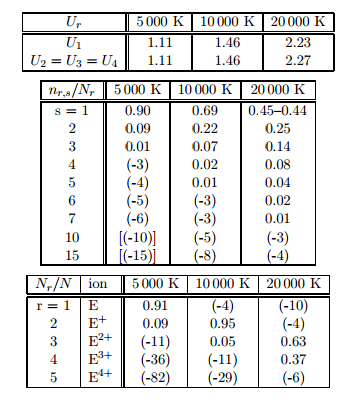
\includegraphics[scale=0.8]{table1.png}
  \caption{Table 1 from reference \cite{cite:ssa}}
\end{figure}
%\begin{table}[H]
 % \centering
  %\caption{}
%  \begin{tabular}{|c|c|c|c|}
%    \hline
%    $U_r$&$5\,000$ K&$10\,000$ K&$20\,000$ K\\\hline
%    $U_1$&1.109&1.456&2.232\\
%    $U_2$&1.109&1.456&2.271\\
%    $U_3$&1.109&1.456&2.272\\
%    $U_4$&1.109&1.456&2.272\\\hline
%  \end{tabular}
%  \begin{tabular}{|c|c|c|c|}
%    \hline
%    $n_{r,s}/N_r$&$5\,000$ K&$10\,000$ K&$20\,000$ K\\\hline
%    $s=1$&0.902&0.687&0.448\\
%    2&0.089&0.215&0.251\\
%  \end{tabular}
%  \label{tab:schadefreude}
%\end{table}
From the table, we see that the Saha and Boltzmann distributions behave differently for different temperature. The Boltzmann population (second table) has the highest population in its lowest state, and decreasing exponentially from there, while the Saha population has its most populated stage shifted from the ground stage for higher temperatures.\\\\
To see why this is, we look at equation \eqref{eq:boltzmann} and equation \eqref{eq:saha}. We see that the Boltzmann law has a negative exponential dependence on temperature, explaining why for increasing $s$, $n_{r,s}/N_r$ decreases exponentially. For the Saha law, the main difference is the factor that is proportional to $\propto T^{3/2}$. This causes the ``peak'' of the exponential to be shifted at higher temperatures.\\\\
One can wonder why ionization can fully deplete a stage, even though excitation puts only a few atoms in levels below the ionization level. I am not sure why, but looking at the Saha law, the only parameter I see that could cause equality between high-level and next-ion population at a given temperature is the electron density $N_e$.

\subsection{Payne curves for schadeenium}
The underlying premise of Payne's analysis, was that one can think, that if TE holds in a stellar atmosphere, the expected strength of a spectral line involving level ($r,s$) scales with the Saha-Boltzmann prediction for the lower level population $n_{r,s}$, even if you don't know how the spectral lines are formed.\\\\
We follow the premise by plotting curves like figure 6 in reference \cite{cite:ssa} for various levels of neutral and ionization stages of E.
\begin{figure}[H]
  \centering
  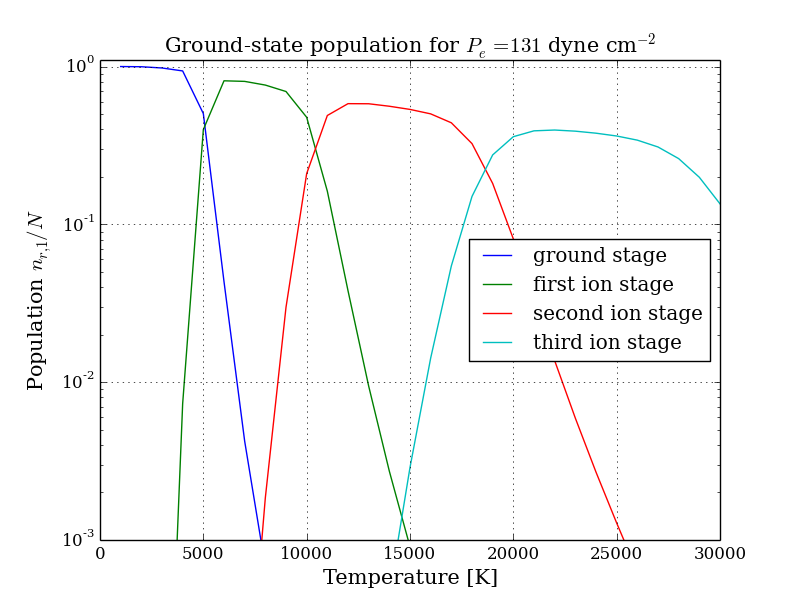
\includegraphics[scale=0.5]{schadeenium_pop.png}
  \caption{Populations for different ionization stages for ground state schadeenium ($s=1$)}
  \label{fig:payne}
\end{figure}
which looks like a Payne-like graph. We see that there are steep flanks on the left and the right side of each peak. This is caused by that there is only a specific temperature range where the specific ionization degree dominates the total population.\\\\
For $T\downarrow 0$, you would assume that most of the population would not be ionized at all, so that $n_{1,1}/N_r \rightarrow 1$, which is what we see in the graph. For $T\uparrow\infty$, we would assume that the element should be fully ionized.\\\\
We can make our plot more like what Payne did by adding curves for higher values of $s$ to the plot.
\begin{figure}[H]
  \centering
  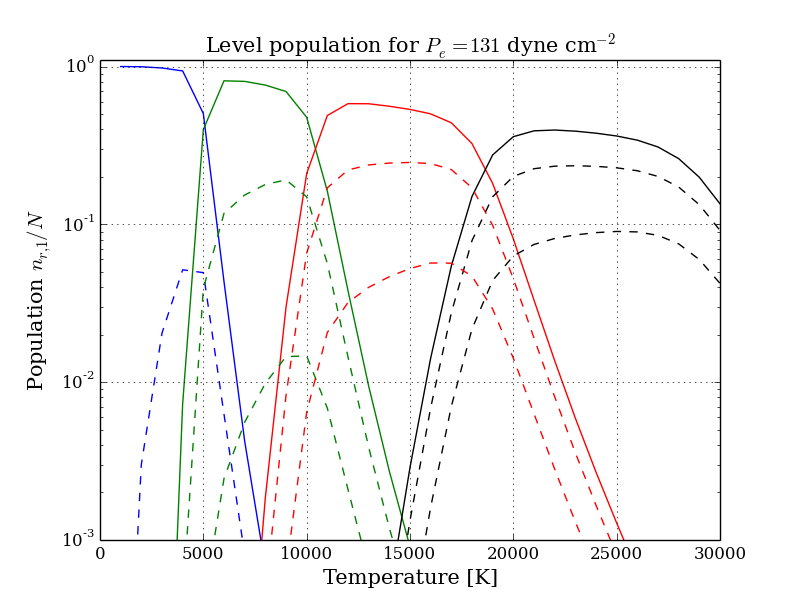
\includegraphics[scale=0.5]{schadeenium_pop_higher.png}
  \caption{Population curves with higher values of $s$ plotted with dashed lines and same color as the ground state population for the specific degree of ionization.}
  \label{fig:payne_lower}
\end{figure}
Looking at figure \ref{fig:payne_lower}, we see that the curves of higher $s$ never overlaps the lower levels, so that the population never exceeds the lower levels. This makes sense, as it requires more energy for an electron to be excited to a higher level $s$, and therefore less should be excited to said level.\\\\
If we were to look at an element with lower/higher ionization energies than E has, we would expect the populations to have even steeper/less steep flanks on the left and right side of the peak, and that the difference between the higher values of $s$ to be larger/smaller.
% high king of skyrim
\subsection{Saha-Boltzmann populations for hydrogen}
Now that we have followed in Payne's footsteps, we have (somewhat) confirmed Payne's conclusion that the Harvard classification of stellar spectra is primarily an ordering with temperature, controlled by Saha-Boltzmann population statistics.\\\\
Since we were only dealing with an hypothetical element E, the natural continuation would be to apply this to actual elements. Luckily, we can write an exact Saha-Boltzmann routine for hydrogen easily.
\begin{itemize}
  \item[-]Its ionization energy is $\chi_1 = 13.598$ eV.
  \item[-]The statistical weights $g_{r,s}$ and level energies $\chi_{r,s}$ are given by
    \begin{align*}
      g_{1,s} &= 2s^2\\
      \chi_{1,s} &= 13.598(1-1/s^2)\;\,\text{eV}
    \end{align*}
  \item[-]Single stage ion stage (bare protons) has $U_2 = g_{2,1} = 1$
\end{itemize}

\subsection{Solar Ca$^+$K versus H$\alpha$: line strength}
Figure 5 (reference \cite{cite:ssa}, p. 10) shows that in solar-type stars the Balmer lines become much weaker than the Ca$^+$K $s=2-1$ line at $\lambda = 3933.7$ Å. Even the principal line of the Balmer sequence, H$\alpha$ ($\lambda = 6563$ Å) gets much weaker than Ca$^+$K in solar-type stars. Figure 9 (reference \cite{cite:ssa}, p. 22) shows how the Ca$^+$K line has a much wider absorption line than H$\alpha$.\\\\
It seems weird that the solar Ca$^+$K line is much stronger than the H$\alpha$ line, even though hydrogen is not ionized in the solar photosphere and low chromosphere, where these lines are formed, and even though the solar Ca/H abundance ratio is only $N_{\text{Ca}}/N_{\text{H}} = 2\cdot10^{-6}$. Why this is the case I'm not fully certain, but since hydrogen has less possible other states that its electron can be in before ionization. Ca$^+$ has more possible configurations of its electrons, and possibly causes slight variance in the wavelength, causing a broadening.\\\\
We can compute the expected strength ratio of these two lines as function of temperature for $P_e = 10^2$ dyne cm$^{-2}$, by combining the actual calcium ionization energies with the schadeenium level structure we created earlier. Since the Ca$^+$K line originates from the ground state, the higher levels are only needed for the partition function, which is approximated within a factor of two by the routines we made for schadeenium.\\\\
Doing this, gives us the following plot for the expected strength ratio between the Ca$^+$K line and the H$\alpha$ line.
\begin{figure}[H]
  \centering
  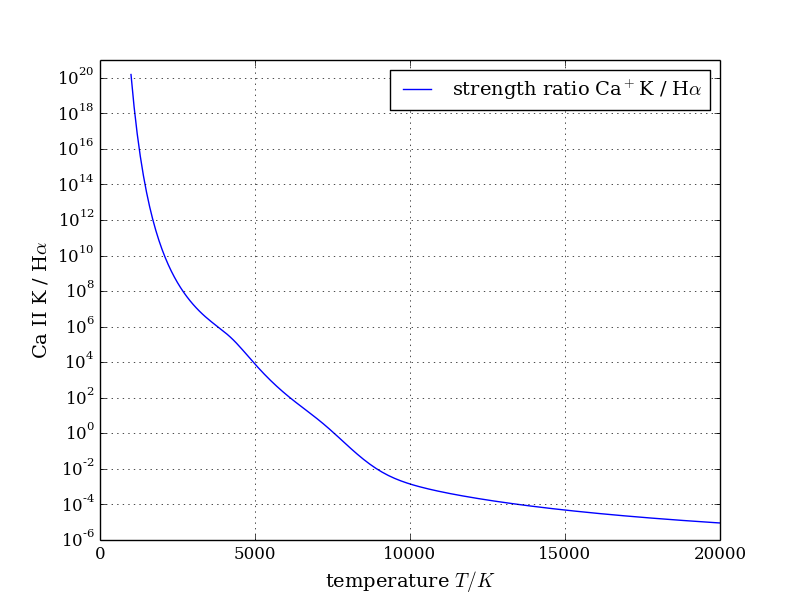
\includegraphics[scale=0.5]{ssa_Ca_Halpha.png}
  \caption{Plot of the expected strength ratio between Ca$^+$K line and H$\alpha$ line, plotted with logarithmic y-axis}
  \label{fig:HCa_strength}
\end{figure}
From figure \ref{fig:HCa_strength} we see that the expected strength ratio decreases exponentially as temperature increases. For temperature $T = 5000$K, we find that the strength ratio is $N_{\text{Ca}}/N_{\text{H}} \approx 7840$, which shows that the Ca$^+$K line is a lot stronger than the H$\alpha$ line at Sun-like temperatures.
\subsection{Solar Ca$^+$K versus H$\alpha$: temperature sensitivity}
Seeing that the lines differ much in their temperature sensitivity, we would be interested in plotting this. We can do this by plotting the relative population changes $(\Delta n_{\text{Ca}}/\Delta T)/n_{\text{Ca}}$ and $(\Delta n_{\text{H}}/\Delta T)/n_{\text{H}}$ for the two lower levels as function of temperature for a small temperature change $\Delta T$. This yields the following plot.
\begin{figure}[H]
  \centering
  \includegraphics[scale=0.5]{temp_sens_Ca_Halpha.png}
  \caption{Plotting the relative population changes for the two lower levels of Ca and H as a function of temperature for a small temperature change $\Delta T$. Overplotted is the relative population variation $n_{\text{Ca}}/\max(n_{\text{Ca}})$ and similarly for hydrogen.}
  \label{fig:temp_sens}
\end{figure}
In figure \ref{fig:temp_sens}, we see that around $T = 5\,600$K, the Ca$^+$K curve has a dip, so that for that specific temperature, the temperature sensitivity of Ca$^+$K is much smaller than the temperature sensitivity of H$\alpha$. For around $T = 9\,500$K, the situation is reversed, and the H$\alpha$ line has a dip. The left flank of each dip has $\Delta n < 0$, while the right flank has $\Delta n > 0$.\\\\
We can study the dips closer by overplotting the variation with temperature of each population in relative units. This is shown in figure \ref{fig:temp_sens} by the dashed lines. The first thing to note, is that the peaks of the relative populations coincide perfectly with the dips in the relative population changes.\\\\
The flank to the left of the peak of the population curves means that the populations is shifting from a lower ionization stage (for Ca) to Ca$^+$ as temperature is increasing. For hydrogen the fraction of atoms in the second level increases as we increase $T$. Similarly, increasing $T$ further beyond the plateau, means that another energy state/ionization stage takes dominance over the relative population.\\\\
The dips in the temperature sensitivity curves means that at the lowest point in the dips, the spectral lines are at their strongest there.

\subsection{Hot stars versus cool stars}
One of the things that can be used to distinguish between ``hot'' and ``cool'' stars, is the temperature at which the hydrogen in stellar photospheres with $P_e = 10^2$ is about 50\% ionized. This transition represents a dividing line between the mechanisms that cause the stellar continuum. In cool stars, there are few free electrons (none from hydrogen), and interactions between the few free electrons and neutral hydrogen atoms, combining them momentarily into H$^-$ ions, dominate the formation of the stellar continuum. We can easily make a plot of the population of the ground state, as a function of the temperature.
\begin{figure}[H]
  \centering
  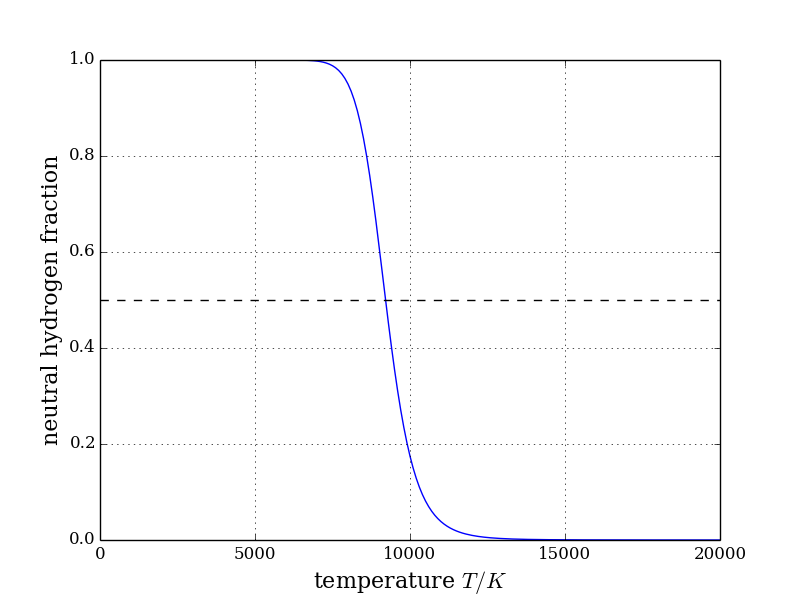
\includegraphics[scale=0.5]{ssa_2_10.png}
  \caption{Plot of the fraction of ground state population versus the temperature. Overplotted, a dashed line at $y=0.5$ to more easily see where the fraction reaches $0.5$.}
  \label{fig:neutral_hydrogen}
\end{figure}
We see from figure \ref{fig:neutral_hydrogen} that as temperature increases, the fraction of neutral hydrogen decreases quite rapidly as $T$ nears $10^3$K. The temperature at which hydrogen is about 50\% ionized is at $T = 9\,212\,$K.

%%%%%%%%%%%%%%%%%%%%%%%%%%%%%%%%%%%%%%%%%%%%%%%%%%%%%%%%%%%%%%%%%%%%%%%%%%%%%%%%
\section{Fraunhofer line strengths and the curve of growth}
In this section we will look at how spectral lines are formed. To adress this issue, we will look at some of the concepts introduced by Marcel Minnaert, many of which are still in use today.\\\\
We will in this task attempt to simulate a radiating body, to see how it compares to observations.
\subsection{The Planck law}
For electromagnetic radiation the counterparts to the material Saha and Boltzmann distributions are the Planck law and its relatives. The Planck function specifies the radiation intensity emitted by a gas or a body in TE as
\begin{align*}
  B_{\lambda}(T) &= \frac{2hc^2}{\lambda^5}\frac{1}{e^{hc/\lambda kT} - 1}\numberthis\label{eq:planck}
\end{align*}
where $h$ is the Planck constant, $c$ the speed of light, $k$ the Boltzmann constant, $\lambda$ the wavelength, and $T$ the temperature.
\\\\
We can plot this against wavelength for different temperatures to see how the Planck curves behave.
\begin{figure}[H]
  \centering
  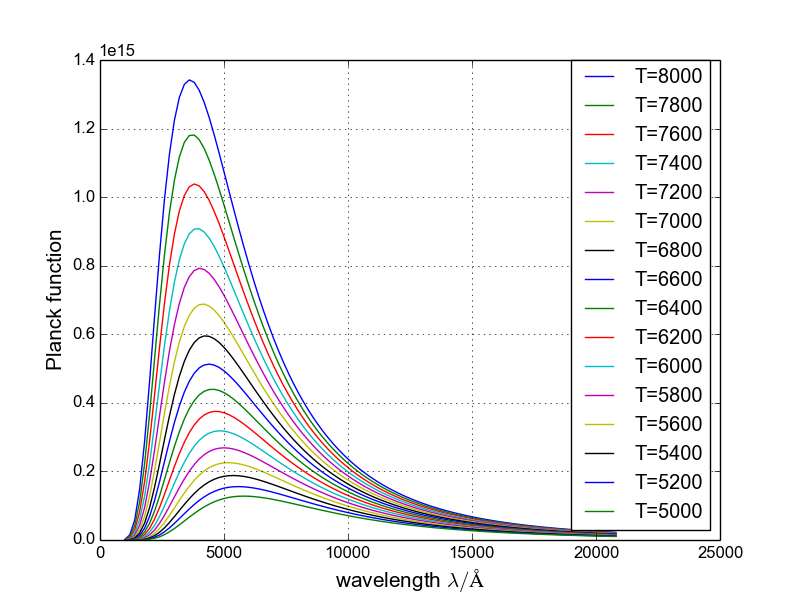
\includegraphics[scale=0.5]{ssa_3_1.png}
  \caption{Planck curves plotted against wavelength in the visible spectrum for different stellar-like temperatures, linear scale}
  \label{fig:planck_linear}
\end{figure}
We see from figure \ref{fig:planck_linear} that the height of the peak increases steeply with temperature. We see that for shorter wavelengths, $B_{\lambda}(T)$ increases much faster (exponentially, Wien regime), than for longer wavelengths (linearly, Rayleigh-Jeans regime). The peak divides the two regimes, and shifts to shorter wavelengths for higher temperatures, as per Wien's displacement law.\\\\
We can plot with logarithmic axis.
\begin{figure}[H]
  \centering
  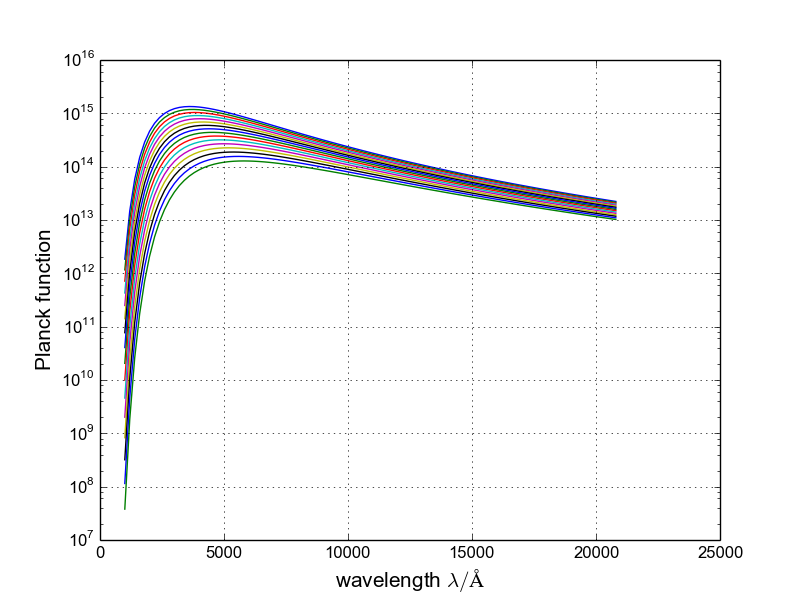
\includegraphics[scale=0.5]{ssa_3_1_logy.png}
  \caption{Plot of the Planck curves, logarithmic y-axis}
  \label{fig:planck_logy}
\end{figure}
We see that in figure \ref{fig:planck_logy}, the y-axis is logarithmic, and looks about how we would expect from figure \ref{fig:planck_linear} when plotted with a logarithmic y-axis. The slope on the righthand side of the peak increases linearly towards the peak.
\begin{figure}[H]
  \centering
  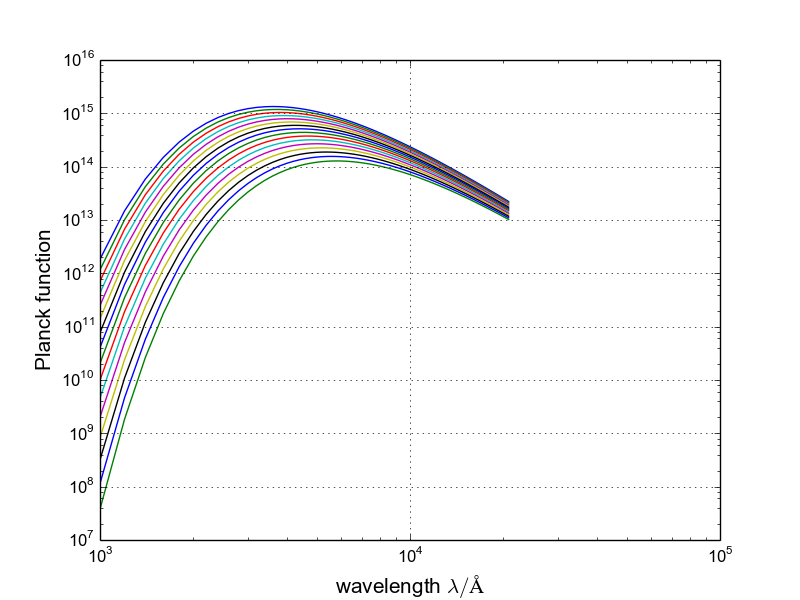
\includegraphics[scale=0.5]{ssa_3_1_loglog.png}
  \caption{Plot of the Planck curves, logarithmic x- and y-axis}
  \label{fig:planck_loglog}
\end{figure}
In figure \ref{fig:planck_loglog}, both axis are logarithmic.

\subsection{Radiation through an isothermal layer}
Just the radiation produced by a gas of temperature $T$ is not enough, we also need the amount of absorption.\\\\
We look at a beam of radiation passing through a layer of gas, where it is attenuated. The weakened beam emerging has an intensity given by
\begin{align*}
  I = I(0)\,e^{-\tau}
\end{align*}
where $\tau$ is the decay parameter specifying the attenuation by absorption in the layer. It is also called optical thickness/opaqueness.\\\\
We add the radiation that originates within the layer itself. This local contribution at a location $x$ within the layer is subsequently attenuated by the remainder of the layer to the right. The total emergent intensity is then given by
\begin{align*}
  I_{\lambda} &= I_{\lambda}(0)e^{-\tau} + \int\limits_0^{\tau}B_{\lambda}[T(x)]\,e^{-(\tau-\tau(x))}\,d\tau(x)
  \intertext{for an isothermal layer, $T$ and therefore $B_{\lambda}(T)$ is independent of $x$, so}
  I_{\lambda} &= I_{\lambda}(0)e^{-\tau} + B_{\lambda}e^{-\tau}\int\limits_0^{\tau}e^{\tau(x)}d\tau(x)\\
  &= I_{\lambda}(0)e^{-\tau} + B_{\lambda}e^{-\tau}\underbrace{\big[e^{\tau(x)}\big]_0^{\tau}}_{e^{\tau}-1}\\
  &= I_{\lambda}(0)e^{-\tau} + B_{\lambda}e^{-\tau}(e^{\tau}-1)
  \intertext{so that the emergent intensity simplifies to}
  I_{\lambda} &= I_{\lambda}(0) + B_{\lambda}\,(1-e^{-\tau})\numberthis\label{eq:emergent_intensity}
\end{align*}
Now that we have an expression for the emergent intensity, we can make a plot of $I_{\lambda}$ for given values $B_{\lambda}$ and $I_{\lambda}(0)$ against $\tau$
\begin{figure}[H]
  \centering
  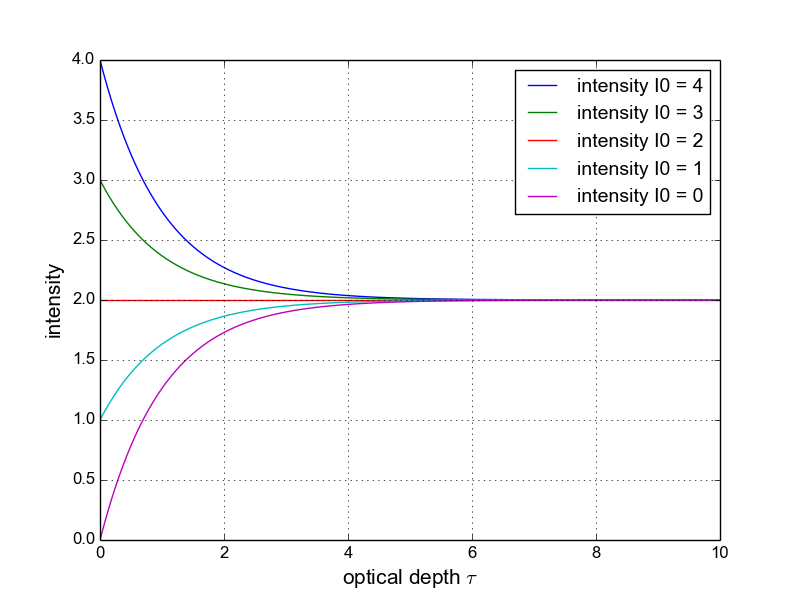
\includegraphics[scale=0.5]{ssa_3_2.png}
  \caption{Plot of the emergent intensity $I_{\lambda}$ for given values $B_{\lambda}=2$ and $I_{\lambda}(0)$ against $\tau$.}
  \label{fig:intensity_linear}
\end{figure}
\begin{figure}[H]
  \centering
  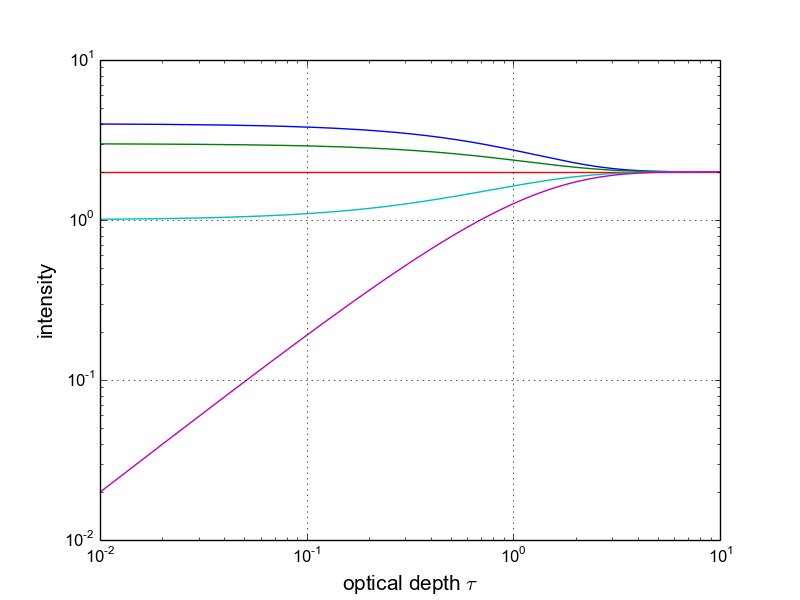
\includegraphics[scale=0.5]{ssa_3_2_log.png}
  \caption{Plot of the emergent intensity for $B_{\lambda}=2$ with logarithmic x,y axis}
  \label{fig:intensity_loglog}
\end{figure}
From looking at figure \ref{fig:intensity_linear} and figure \ref{fig:intensity_loglog}, we can see how $I_{\lambda}$ depends on $\tau$.\\\\
\begin{itemize}
  \item[-]For $\tau \ll 1$, illustrated well in figure \ref{fig:intensity_loglog}, there is very little change in the intensity of the beam as it passes through the layer. For $I_{\lambda}(0) = 0$, as we increase $\tau$, the emergent intensity increases steadily towards the value of $B_{\lambda}$. For $I_{\lambda}(0) > B_{\lambda}$, $I_{\lambda}$ decreases as $\tau$ is increased. A layer where $tau\ll 1$ is called ``optically thin'', since the beam goes through the layer mostly unchanged.
  \item[-]For $\tau \gg 1$, we see in figure \ref{fig:intensity_linear} that independently of the initial intensity, the emergent intensity $I_{\lambda}$ converges to the radiation contributed by the layer $B_{\lambda}$. Such a layer is called ``optically thick'', as the beam going through the layer will be fully absorbed by the layer, so that the radiation emitted by the layer is all we see when we look at it.
\end{itemize}

\subsection{Spectral lines from a solar reversing layer}
We will now apply the above result for an isothermal layer to a simple model in which the Fraunhofer lines in the solar spectrum are explained by a ``reversing layer''.
\subsubsection*{Schuster-Schwarzschild model}
In this model, we have a few basic assumptions
\begin{itemize}
  \item[-]The continuous radiation, without spectral lines, is emitted by the stellar surface and irradiates a separate layer with the intensity
    \begin{align*}
      I_{\lambda}(0) &= B_{\lambda}(T_{\text{surface}})\numberthis\label{eq:ss_basic}
    \end{align*}
  \item[-]This layer sits as a shell around the star and causes attenuation and local emission only at the wavelengths of spectral lines.
  \item[-]The star is optically thick ($\tau\gg1$), so that the surface radiates with the $\tau\gg1$ solution $I_{\lambda} = B_{\lambda}(T_{\text{surface}})$ of equation \eqref{eq:emergent_intensity}. Depending on atom concentration, the shell may be optically thin or thick.
  \item[-]The line-causing atoms in the shell have temperature $T_{\text{layer}}$ so that the local production of radiation in the layer at the line wavelengths is given by $B_{\lambda}(T_{\text{layer}})\Delta\tau(x)$.
\end{itemize}
The emergent radiation at the line wavelengths is then given by combining \eqref{eq:emergent_intensity} and \eqref{eq:ss_basic}
\begin{align*}
  I_{\lambda} &= B_{\lambda}(T_{\text{surface}})\,e^{-\tau_{\lambda}}+B_{\lambda}(T_{\text{layer}})\,(1-e^{-\tau_{\lambda}}) \numberthis\label{eq:ss_full}
\end{align*}

\subsubsection*{Voigt profile}
The opaqueness $\tau$ in \eqref{eq:ss_full} has an index $\lambda$ because it varies over the spectral line. We will be looking at the broadening distribution caused by Coulomb interactions by neighboring particles. This broadening distribution is described by
\begin{align*}
  \tau(u) &= \tau(0)\,V(a,u)\numberthis\label{eq:voigt}
\end{align*}
where $V$ is called the Voigt function and $u$ measures the wavelength separation $\Delta \lambda = \lambda-\lambda(0)$ from the center of the line at $\lambda=\lambda(0)$ in dimensionless units
\begin{align*}
  u \equiv \Delta\lambda/\Delta\lambda_{\text{D}}
\end{align*}
where $\Delta\lambda_{\text{D}}$ is the Doppler width
\begin{align*}
  \Delta\lambda_{\text{D}} \equiv\frac{\lambda}{c}\sqrt{2kT/m}
\end{align*}
The Voigt function is defined as
\begin{align*}
V(a,u)\equiv \frac{1}{\Delta\lambda_{\text{D}}\sqrt{\pi}}\,\frac{a}{\pi}\int_{-\infty}^{+\infty}\,\frac{e^{-y^2}}{(u-y)^2 + a^2}dy \numberthis\label{eq:voigt_hell}
\end{align*}
The Voigt function represents the convolution of a Gauss profile with a Lorentz profile, and therefore has a Gaussian shape close to line center. We can find a reasonable approximation to the full Voigt function
\begin{align*}
  V(a,u) \approx \frac{1}{\Delta\lambda_{\text{D}}\sqrt{\pi}}\bigg[e^{-u^2} + \frac{a}{\sqrt{\pi}u^2}\bigg] \numberthis\label{eq:voigt_approx}
\end{align*}
We can plot the Voigt function \eqref{eq:voigt_hell} for $u = -10$ to $u = +10$ and for $a$ ranging between $a=0.001$ and $a=1$ 
\begin{figure}[H]
  \centering
  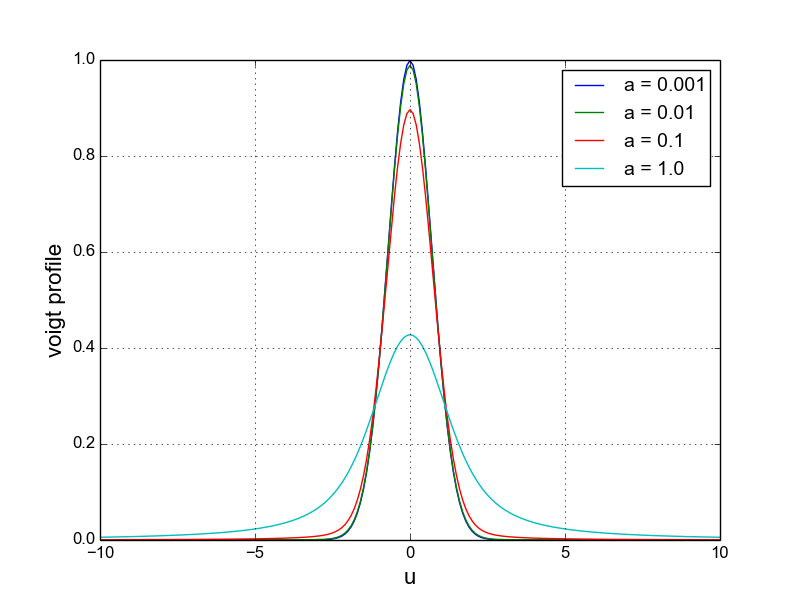
\includegraphics[scale=0.5]{ssa_voigt.png}
  \caption{Plot of the Voigt function \eqref{eq:voigt_hell} for $u=-10$ to $u=10$ and $a=0.001$ to $a=1$}
  \label{fig:voigt}
\end{figure}
\begin{figure}[H]
  \centering
  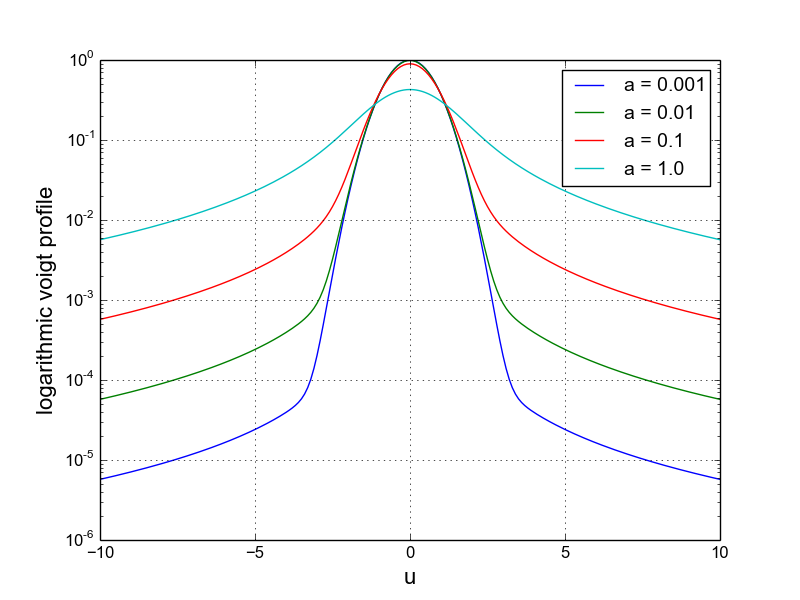
\includegraphics[scale=0.5]{ssa_voigt_ylog.png}
  \caption{Plot of the Voigt function \eqref{eq:voigt_hell} with logarithmic y-axis}
  \label{fig:voigt_ylog}
\end{figure}
We inspect the far wings of the profile by looking at figure \ref{fig:voigt_ylog}. For $u$ far from the center of the profile $u=0$, we see in our approximation, eq. \eqref{eq:voigt_approx}, that the second term ($a/\sqrt{\pi}u^2$) is proportional to $a$, so increasing $a$ would make this term larger, resulting in extended/wider wings, which is what we see in the plot.

\subsubsection*{Emergent line profiles}
We can now compute and plot stellar spectral line profiles by combining \eqref{eq:ss_full} and \eqref{eq:voigt}. Again using dimensionless $u$ units for the wavelength scale, thereby avoiding having to calculate the Doppler width $\Delta\lambda_{\text{D}}$.
\begin{figure}[H]
  \centering
  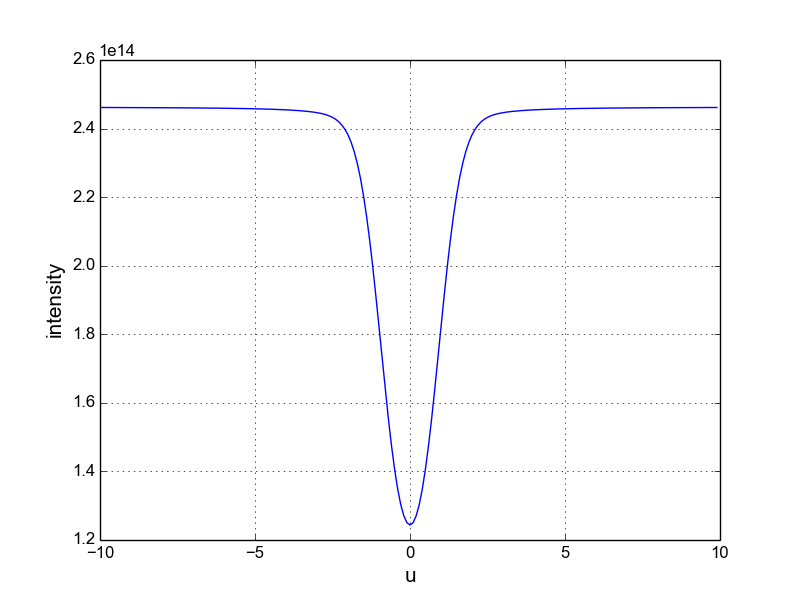
\includegraphics[scale=0.5]{ssa_3_3_1.png}
  \caption{Plot of profile $I$ against $u$ for $\tau(0) = 1$, $T_{\text{surface}} = 5600$ K, $T_{\text{layer}}=4200$ K, $a=0.1$, $\lambda=5000$ Å}
  \label{fig:ssa_3_3_1}
\end{figure}
Then we study the appearance of the line in the spectrum as a function of $\tau(0)$ over the range $\log\tau(0) = -2$ to $\log\tau(0) = 2$.
\begin{figure}[H]
  \centering
  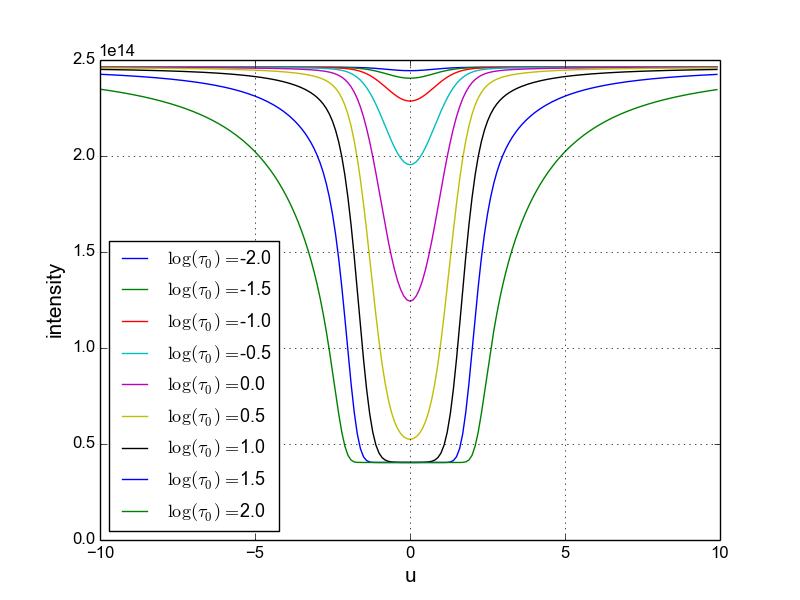
\includegraphics[scale=0.5]{ssa_3_3_2.png}
  \caption{Plot of $I$ against $u$ for a range of $\tau(0)$, $T_{\text{surface}} = 5600$ K, $T_{\text{layer}}=4200$ K, $a=0.1$, $\lambda=5000$ Å}
  \label{fig:ssa_3_3_2}
\end{figure}
Looking at figure \ref{fig:ssa_3_3_2}, we can hopefully unveil some of the properties of the line profiles.\\\\
For $\tau\ll1$, the profiles are very weak absorption lines. For example, for $\log\tau(0) = -2$, the profile is almost a straight line, indicating that the reversing layer is optically thin, and $\tau_{\lambda} \ll 1$ is satisfied for all $\lambda$. Increasing $\tau(0)$ slightly, we see that the profile gets deeper, and the wings slowly get wider.\\\\
This continues until the profile reaches a low-intensity saturation limit for $\tau\gg1$. When $\tau(0)$ gets large, we recall from earlier that the emergent radiation ends up following the radiation emitted by the layer itself. Due to this, there is a limit to how low the intensity can get in the center of the spectral line for an optically thick layer, since we will at some point start seeing the radiation from the layer.\\\\
The line wings only develop for very large $\tau(0)$, as $\tau_{\lambda}$ will decrease the further out from $u=0$ we go, but much more slowly than for lower $\tau(0)$, so there will be a natural broadening of the line due to this.\\\\
We can attempt to study the dependence of these line profiles on wavelength by repeating the above for $\lambda = 2\,000$ Å, and $\lambda = 10\,000$ Å.
\begin{figure}[H]
  \centering
  \begin{subfigure}[b]{0.49\textwidth}
    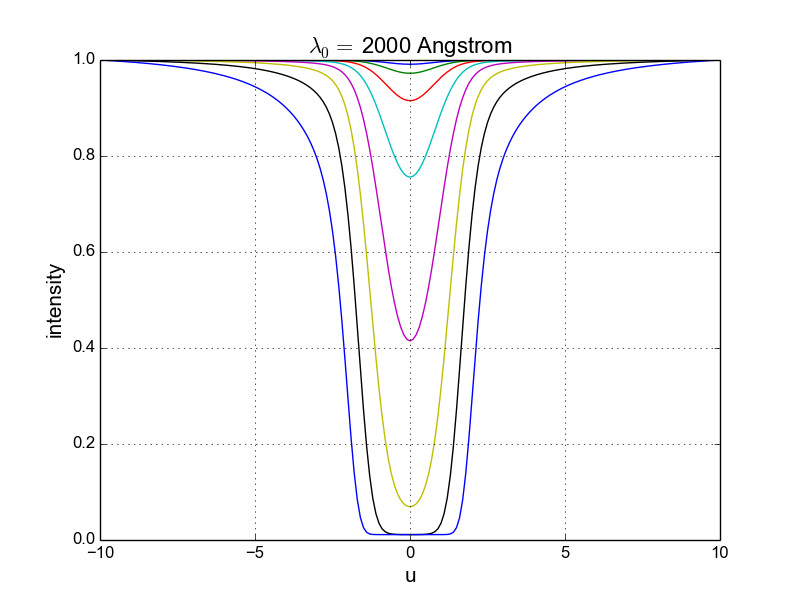
\includegraphics[width=\textwidth]{ssa_3_3_wave_1.png}
    \caption{$\lambda_0 = 2\,000$ Å}
  \end{subfigure}
  \begin{subfigure}[b]{0.49\textwidth}
    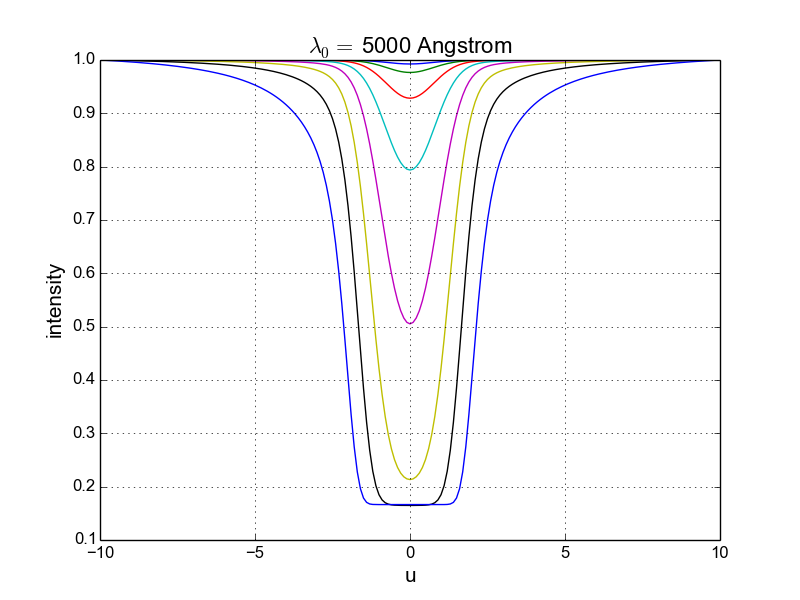
\includegraphics[width=\textwidth]{ssa_3_3_wave_2.png}
    \caption{$\lambda_0 = 5\,000$ Å}
  \end{subfigure}
  \begin{subfigure}[b]{0.49\textwidth}
    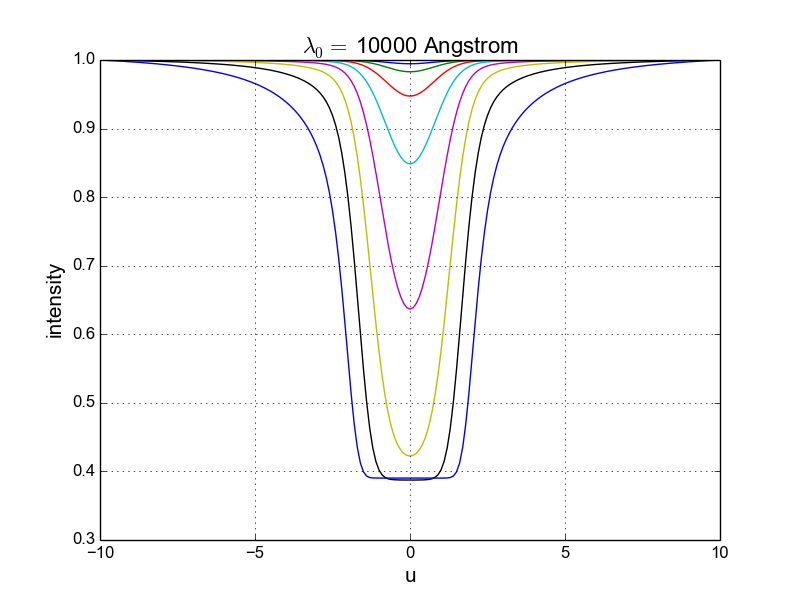
\includegraphics[width=\textwidth]{ssa_3_3_wave_3.png}
    \caption{$\lambda_0 = 10\,000$ Å}
  \end{subfigure}
  \caption{Profile shapes for various wavelengths}
  \label{fig:wave}
\end{figure}
The figures in figure \ref{fig:wave} is already plotted with scaled to the local continuum intensity $I_{\lambda}/I_{\text{cont}}$, so unless new plots were to be made without the scaling, it is hard to tell much about the continuum intensity.\\\\
We see from figure \ref{fig:wave}, that increasing the wavelength causes ratio between the limit value and continuum value increases.

\subsection{The equivalent width of spectral lines}
The profile plots in the last section demonstrate that the growth of the absorption feature in the spectrum for increasing $\tau(0)$ is faster for small $\tau(0)$ then when it saturates for larger $\tau(0)$. From Minnaert, we introduce the equivalent width $W_{\lambda}$ as a line-strength parameter to measure this growth quantitatively.
\begin{align*}
  W_{\lambda} \equiv \int\frac{I_{\text{cont}}-I(\lambda)}{I_{\text{cont}}}d\lambda
\end{align*}
\begin{figure}[H]
  \centering
  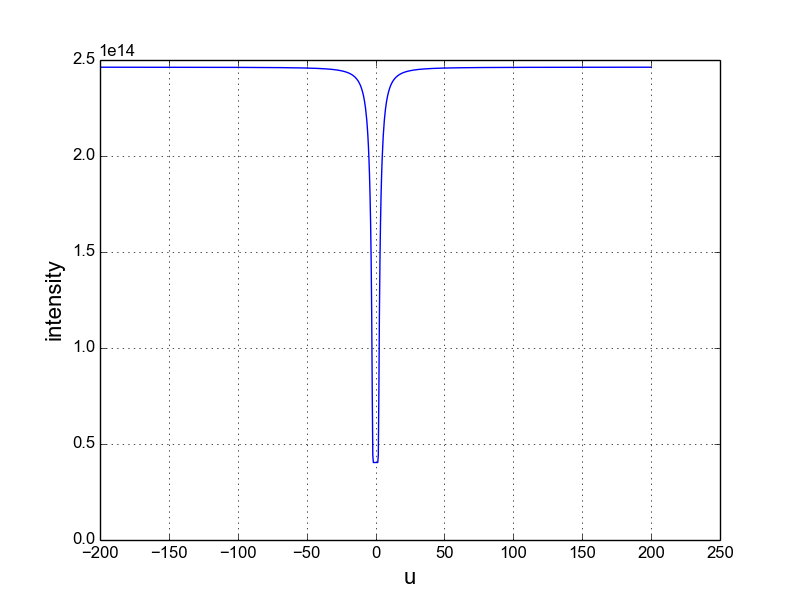
\includegraphics[scale=0.5]{ssa_3_4_1.png}
  \caption{Plot of equivalent width line depth}
  \label{fig:eqw}
\end{figure}
\begin{figure}[H]
  \centering
  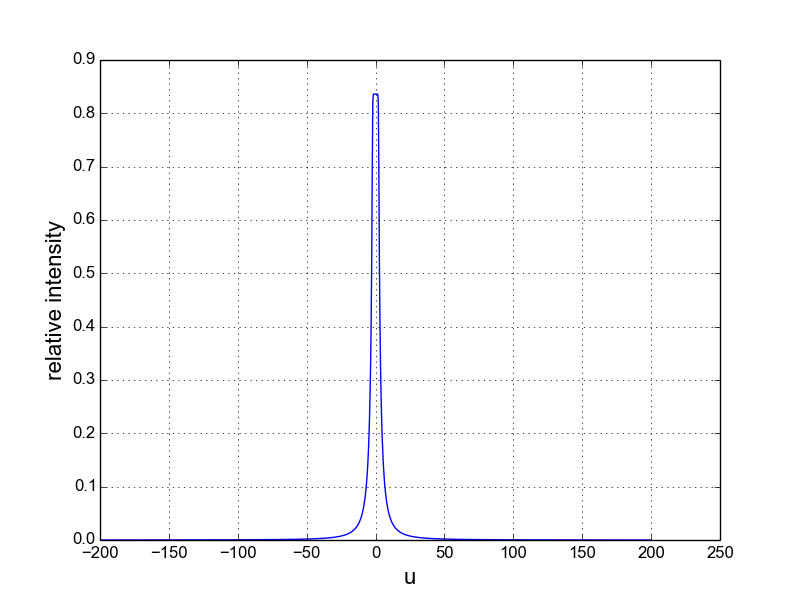
\includegraphics[scale=0.5]{ssa_3_4_2.png}
  \caption{Line depth in relative units}
  \label{fig:rel_width}
\end{figure}
We compute the equivalent width from figure \ref{fig:rel_width}, and find the equivalent width to be $W_{\lambda} = 7.54$.\\\\
We can check how this matches by integrating the plot in figure \ref{fig:eqw}, which I haven't done.
\subsection{The curve of growth}
The idea behind equivalent width,is that the amount of spectral blocking should be a direct measure of the number of atoms in the reversing layer. Our profile plots illustrate that the profile growth is only linear with $\tau(0)$ for $\tau(0)\ll1$. To show the full dependence, we plot the ``curve of growth'': the growth of the line strength with the line-causing particle density.

\begin{figure}[H]
  \centering
  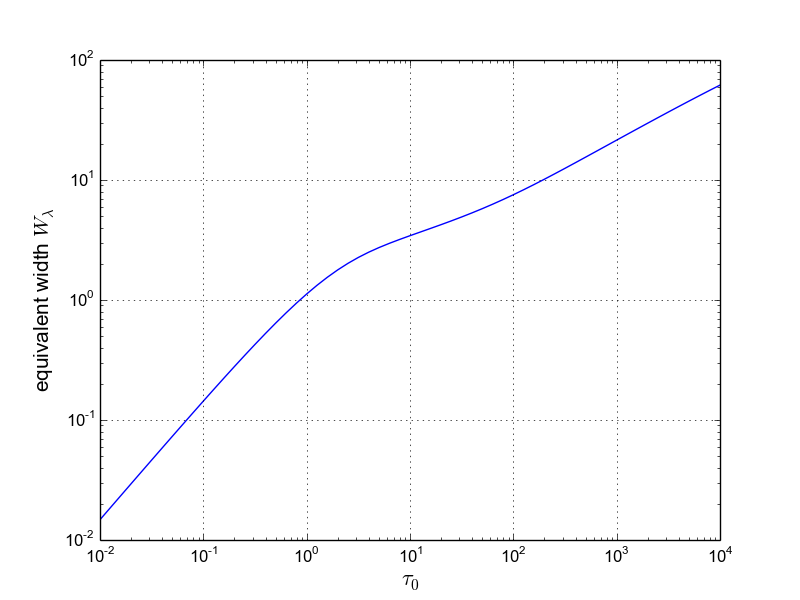
\includegraphics[scale=0.5]{ssa_3_5.png}
  \caption{Curve of growth}
  \label{fig:curve}
\end{figure}
We see that figure \ref{fig:curve} is split into three regimes:
\begin{itemize}
  \item[-]Before saturation: Low absorption, small optical depth
  \item[-]''During'' saturation: Doppler wings barely change for a while
  \item[-]After saturation: Collisional broadening takes over eventually
\end{itemize}
It makes a fair bit of sense that the curve grows fastest in the first part, as the layer is optically thin, so equivalent width of the line increases fast. Not sure which parameter that controls the location of the onset of the third part.\\\\
If we want to make emission lines instead of absorption lines, then we should switch the temperatures of the surface $T_{\text{surface}}$ and layer $T_{\text{layer}}$.
\begin{figure}[H]
  \centering
  \begin{subfigure}[b]{0.49\textwidth}
    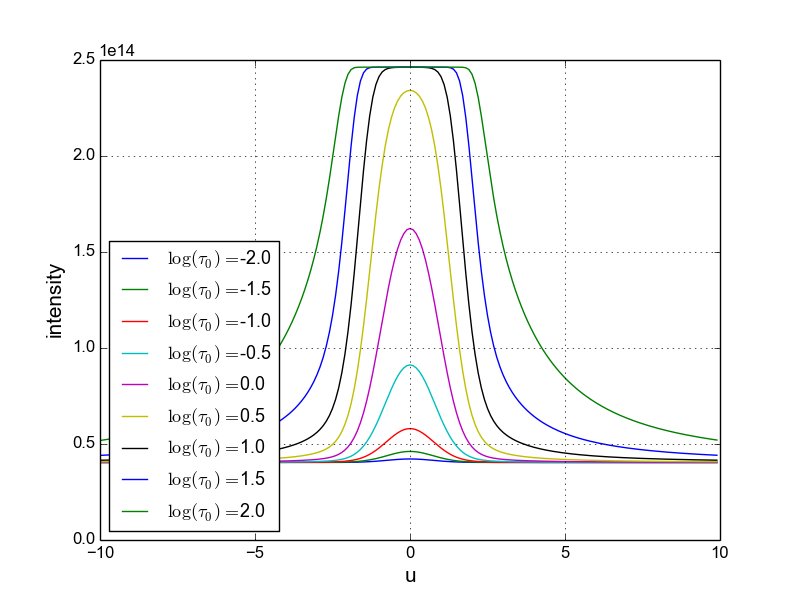
\includegraphics[width=\textwidth]{ssa_3_5_1.png}
    \caption{Emission profile}
  \end{subfigure}
  \begin{subfigure}[b]{0.49\textwidth}
    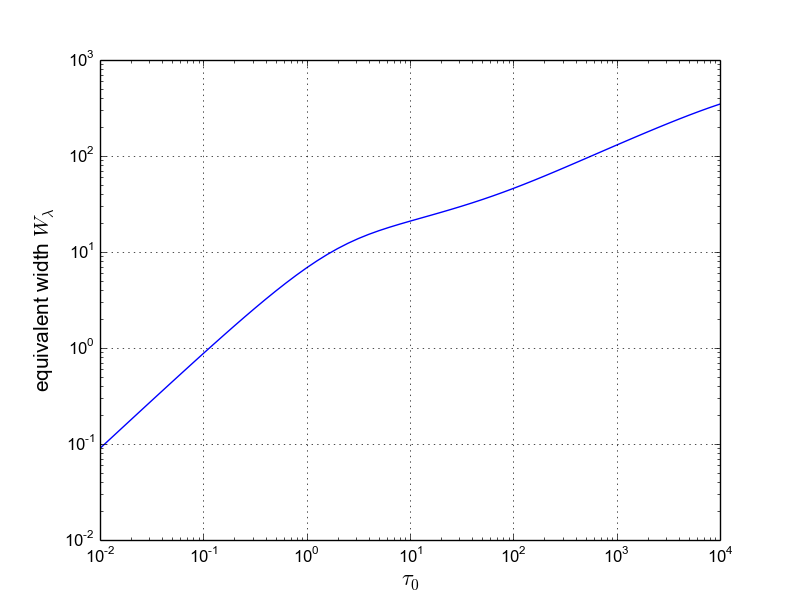
\includegraphics[width=\textwidth]{ssa_3_5_2.png}
    \caption{Emission-line curve of growth}
  \end{subfigure}
  \caption{Plot of emission profiles and an emission-line curve of growth}
\end{figure}
We see that the emission profiles are pretty much just the same as the absorption profiles inverted, which is to be expected. The curve of growth remains unchanged, which is not very surprising as the equivalent width of an emission line should be the same as an absorption line under similar situations.

\section{Appendix}
\subsection{Saha-Boltzmann tables}
\verbatiminput{table.txt}
\subsection{Code}
\subsubsection{For schadeenium}
\lstinputlisting[language=Python]{ssa2.py}
\subsubsection{For hydrogen}
\lstinputlisting[language=Python]{ssa_hydrogen.py}
\subsubsection{For Ca and Halpha line}
\lstinputlisting[language=Python]{ssa_ca_temp_sens.py}
\lstinputlisting[language=Python]{ssa_2_10.py}
\subsubsection{Task 3}
\lstinputlisting[language=Python]{ssa_3_1.py}
\lstinputlisting[language=Python]{ssa_3_2.py}
\lstinputlisting[language=Python]{ssa_3_3.py}
\lstinputlisting[language=Python]{ssa_3_4.py}
\lstinputlisting[language=Python]{ssa_3_5.py}
\lstinputlisting[language=Python]{ssa_3_emission.py}

\begin{thebibliography}{40}
  \bibitem{cite:ssa}Stellar spectra A: basic line formation\\\href{http://www.uio.no/studier/emner/matnat/astro/AST4310/h12/undervisningsmateriale/ssa.pdf}{http://www.uio.no/studier/emner/matnat/astro/AST4310/h12/undervisningsmateriale/ssa.pdf}
\end{thebibliography}
\end{document}
